\chapter{Análisis y diseño del sistema}

En este capítulo se expone el análisis de requisitos funcionales, la arquitectura software, la base de datos y la interfaz del usuario.

\section{Requisitos del sistema}
\label{section-requisitos}

Seguidamente (véase tabla \ref{tab:etiqueta_tabla}) se presentan, en modo de tabla, los principales requisitos del sistema que se han acordado con la empresa.

% Tabla con los requisitos del sistema

% \begin{table}[!h]
% \centering
% \begin{tabular}{|p{1cm}|p{14cm}|}
\begin{longtable}{|p{1cm}|p{14cm}|}
	\hline
	\textbf{ID} & \textbf{Requisito} \\
	\hline
	RF-1 	& 	Un usuario iniciará sesión en el sistema utilizando usuario, contraseña y puesto. \\
	\hline
	RF-2	&	Un usuario podrá cerrar su sesión.	\\
	\hline
	RF-3	&	El sistema permitirá al usuario navegar en la aplicación mediante un menú lateral. \\
	\hline
	RF-4	&	El sistema mostrará al usuario un listado de plantas del edificio. \\
	\hline
	RF-5	&	El sistema mostrará al usuario el número total de alarmas y presencias activas en cada planta. \\
	\hline
	RF-6	&	El sistema permitirá al usuario elegir una planta y ver la información de alertas correspondiente a esa planta. \\
	\hline
	RF-7	&	El sistema mostrará al usuario un carrusel con las alertas de la planta seleccionada. \\
	\hline
	RF-8	&	El sistema mostrará al usuario la información del paciente de las alarmas activas y el lugar y momento en el que se han disparado. \\
	\hline
	RF-9	&	El sistema mostrará al usuario la información del trabajador de las presencias identificadas activas y el lugar y momento en el que se han producido. \\
	\hline
	RF-10	&	El sistema mostrará al usuario el plano de la planta seleccionada. \\
	\hline
	RF-11	&	El sistema destacará al usuario en el plano las habitaciones que tengan alguna alerta en activo. \\
	\hline
	RF-12	&	El sistema mostrará al usuario el listado de alarmas pendientes, sin filtrado por planta, indicando el tipo de alarma. \\
	\hline
	RF-13	&	El sistema mostrará al usuario el número total de alarmas y presencias. \\
	\hline
\caption{Requisitos funcionales del sistema}
\label{tab:etiqueta_tabla}
\end{longtable}
	% \end{tabular}
% \end{table}

\section{Arquitectura software del sistema}

% Explicar la arquitectura final del sistema


Para ver las relaciones entre el software y su entorno (dónde se despliega y ejecuta) se utiliza una vista de distribución estilo despliegue. Se puede ver en la \textit{Figura 2.1}. \newline

\begin{figure}[!h]
    \centering
    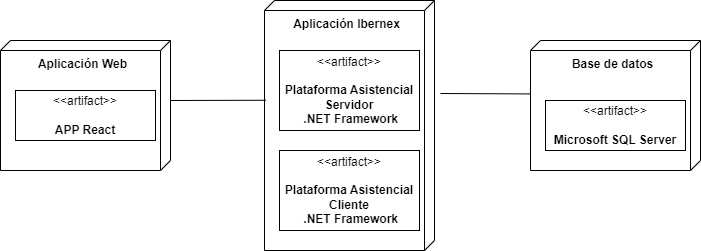
\includegraphics[width=0.8\textwidth,height=6cm]{Imagenes/Arquitectura_Sistema}
    \caption{Diagrama de despliegue}
    \label{fig:despliegue}
\end{figure}

La arquitectura completa respecto a lo que ha estado relacionado con el proyecto es la que se ve en la figura. No obstante lo que se ha implementado ha sido completamente la aplicación web y por otro lado se ha modificado y añadido funcionalidad a la Plataforma Asistencial Servidor de la aplicación de Ibernex. \newline

El ámbito del despliegue del sistema será en una red de área local (LAN) ya que serviría para una residencia u hospital en el que se instalaría el sistema configurando la base de datos correspondiente a la información de los pacientes del centro. \newline


TODO: Terminar de explicar la arquitectura final del sistema consultando con Carlos para hacerlo correctamente respecto a la parte de Ibernex\\

% Explicar que yo mayormente trabajo con PAServidor y qé es, que PACliente no lo toco para nada pero está dentro de la app y para qué lo utilizo.

% Añadir los terminales en el diagrama conectándolo con la aplicación de Ibernex.

% Hacer referencia al Anexo donde se expliquen las alternativas que se plantearon
La arquitectura aquí expuesta es la elegida entre las distintas opciones barajadas que se pueden ver con detalle en el \hyperref[anexo-a]{Anexo A}.


\section{Base de datos}

% Explicar qué partes de la base de datos utilizo de su sistema y con diagramas

TODO: explicar qué tablas de la base de datos utilizo de su sistema y adjuntaré  diagramas creados con la aplicación Microsoft SQL Server Management. \\

\section{Interfaz de usuario}

% Poner la interfaz final del usuario cuando esté terminada

TODO: Poner la interfaz final del usuario cuando esté terminada
